\section{Physikalische Grundlagen}

\subsection{Das Prinzip der Beugung und der Interferenz}
Unter dem Phänomen der Beugung versteht man die Ablenkung von Wellen an Hindernissen. Nach dem Huygenschen Prinzip entsteht an jedem Objekt, an dem das Licht gebeugt wird, eine Kugelwelle. Dadurch kann sich die Welle in einem Bereich des Raumes ausbreiten, welcher auf geradem Wege durch das Objekt versperrt wäre. Im folgenden Bild wird dieses Prinzip am Beispiel eines Spaltes schematisch dargestellt.

\begin{figure}[h]
\begin{center}
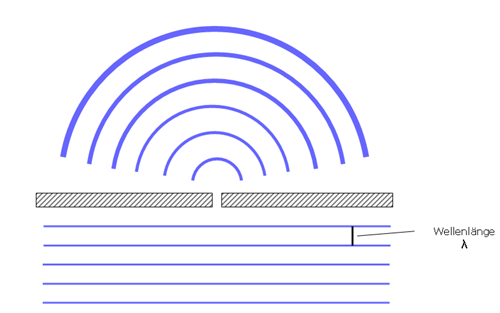
\includegraphics[scale=0.5]{img/holo1}
\caption{Beugung an einem Spalt}
\end{center}
\end{figure}

Entstehen Kugelwellen an mehreren Hindernissen kommt es zwischen diesen zur Interferenz. Bei der Überlagerung von zwei Wellenbergen oder -tälern addieren sich diese und werden entsprechend hoch bzw. tief (konstruktive Interferenz). Treffen ein Wellenberg und ein -tal aufeinander, löschen sich diese aus. (destruktive Interferenz).
Im folgenden Bild wird dies nochmal beispielhaft dargestellt.

\begin{figure}[h]
\begin{center}
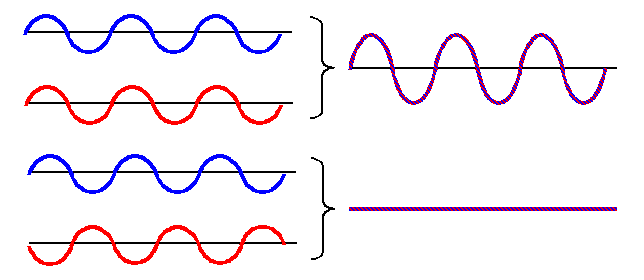
\includegraphics[scale=0.5]{img/holo2}
\caption{Konstruktive und destruktive Interferenz}
\end{center}
\end{figure}

\subsection{Kohärenz}
Der Begriff der Kohärenz beschreibt heutzutage die Gesamtheit der Korrelationseigenschaften von Licht. Dabei unterscheidet man zwischen der räumlichen und der zeitlichen Kohärenz. Das liegt daran, dass es u.a. jeweils messtechnisch gut realisiert werden kann.

\subsubsection{Die räumliche Kohärenz}
Bei der räumlichen Kohärenz bringt man das Licht dazu, räumlich verschoben mit sich selber zu interferieren. Dabei benutzt man das Young'sche Doppelspaltexperiment. Dabei schickt man einen Lichtstrahl durch ein Gitter. Laut dem Huygenschen Prinzip entsteht bei der Beugung von Licht an einem Hindernis eine Kugelwelle. Demzufolge Interferieren hinter einem Gitter die entstandenen Kugelwellen miteinander und erzeugen somit das Interferenzmuster. Der Abstand der einzelnen Spalten verursacht dabei den Gangunterschied der einzelnen Kugelwellen (siehe Abb. 3). 

\begin{figure}[h]
\begin{center}
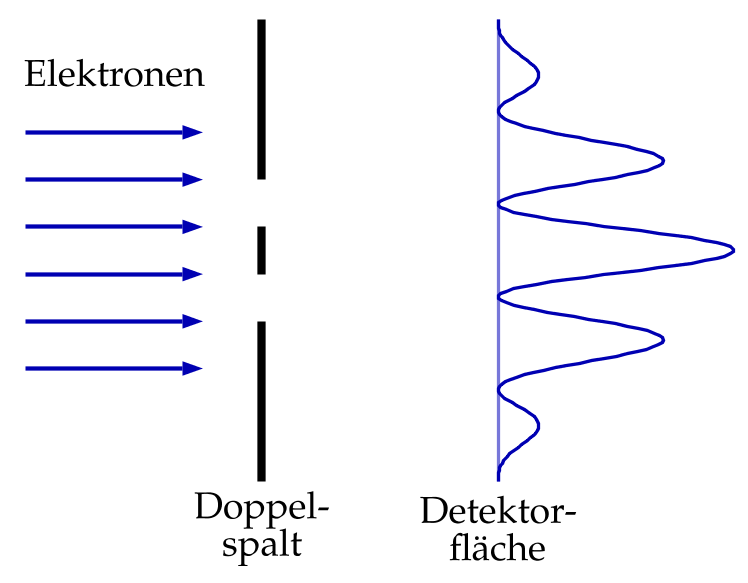
\includegraphics[scale=0.8]{img/holo3}
\caption{Schematische Darstellung eines Michelson-Interferometers}
\end{center}
\end{figure}

\subsubsection{Die zeitliche Kohärenz}
Man kann einen Lichtstrahl in einem Michelson-Interferometer zeitverschoben mit sich selber interferieren lassen. Dabei wird das Licht in einem Strahlteiler in zwei Strahlen aufgeteilt. Der erste Strahl wird in einem feststehenden Spiegel direkt zurück reflektiert, während der zweite Strahl an einem verschiebbaren Spiegel reflektiert wird. Die beiden reflektierten Strahle werden am Strahlteiler jeweils erneut aufgeteilt. Jeweils ein Teil der Strahlen wird auf einen Schirm gestrahlt, während der jeweils andere Teil der Strahlen zur Lichtquelle zurück gelangt. 

\begin{figure}[h]
\begin{center}
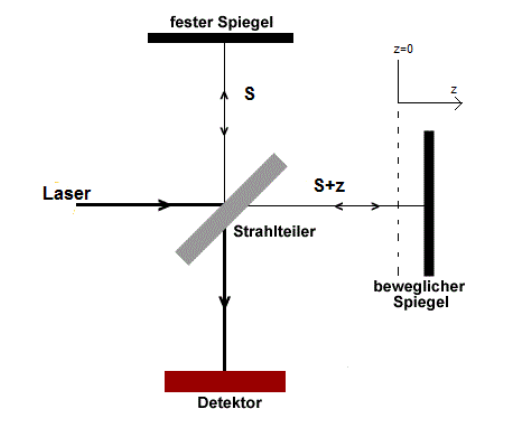
\includegraphics[scale=0.5]{img/holo4}
\caption{Schematische Darstellung eines Michelson-Interferometers}
\end{center}
\end{figure}
 
\newpage
\subsection{Die Eigenschaften eines Helium-Neon-Lasers}

\subsection{Optische Gitter}

\subsubsection{Das Sinusgitter}

\subsubsection{Rechteckgitter}

\subsubsection{Transmissions- und Reflexionsgitter}

\subsection{Das Prinzip der optischen 
Informationsspeicherung in Hologrammen}
Im Grunde wird ein Hologramm durch zwei kohärente Laserstrahlen in einem lichtempfindlichen Medium gebildet. Dabei benutzt man, dass einer dieser Laserstrahlen an einem Objekt gestreut wird (der sog. Objektstrahl) und der andere Laserstrahl (der sog Referenzstrahl) mit diesem ein Interferenzmuster erzeugt.
Wird nun dieses Interferenzmuster auf einer Photoplatte gespeichert und entwickelt, erhält man ein Intensitätsmuster bzw ein Amplituden- oder Phasenhologramm, das alle nötigen Informationen enthält welche zur Rekonstruktion eines räumlichen Bildes des Objekts nötig sind.

\newpage
\subsection{Verwendete Arbeitsmaterialien}
\begin{itemize}
\item schwingungsgedämpfter Tisch 
\item He-Ne-Laser, 10 mW, pol., rot: $\lambda = 632.8$ nm, mit Justierhalterung und Netzgerät 
\item Filterhalterung, dazu: Graufilter in verschiedenen Dichten 
\item Wedge-Filter, zirkular (variabler Strahlteiler) 
\item Strahlteiler (1:1) 
\item 2 Achromaten $f = 400$ mm ($D = 50$ mm) 
\item 2 Achromaten $f = 160$ mm ($D = 40$ mm) 
\item 4 Planspiegel 
\item 2 justierbare Raumfilter mit Mikroskopobjektiv (10x; $f = 16.9$ mm) und 15$\mu$m Lochblende oder Mikroskopobjektiv (16x; $f = 10.8$ mm) und 25 $\mu$m Lochblende 
\item 2 Irisblenden D/A 37.0 mm, $D_{max} = 25.0$ mm 
\item 2 Irisblenden D/A 70.0 mm, $D_{max} = 50$ mm 
\item Elektronischer Verschluss mit Verschlusskontrolleinheit 
\item Belichtungsmesser 
\item 1 Fotodiode, Kabel, Stromverstärker, Oszilloskop, Rechner 
\item Filmmaterial: Slavich PFG-01, dazu: Planfilmhalterung, 
\item Schirme 
\item Dunkelkammer mit entsprechender Ausstattung 
Zu allen optischen Komponenten gehören Montagestäbe, Halterungen und Magnethalter. 
\end{itemize}